\documentclass{article}
\usepackage{graphicx} % Required for inserting images
\usepackage{amsmath}
\usepackage[utf8]{inputenc}
\usepackage[T1]{fontenc}
\usepackage{csquotes}
\usepackage[french]{babel}
\usepackage[a4paper, left=1in, right=1in, top=1in, bottom=1in]{geometry} % Adjust the total width and height
\usepackage[
backend=biber,
style=alphabetic,
]{biblatex}
\usepackage{algorithm}
\usepackage{algpseudocode}

\renewcommand{\algorithmicif}{\textbf{si}}
\renewcommand{\algorithmicthen}{\textbf{alors}}
\renewcommand{\algorithmicelse}{\textbf{sinon}}
\renewcommand{\algorithmicwhile}{\textbf{tant que}}
\renewcommand{\algorithmicdo}{\textbf{faire}}
\renewcommand{\algorithmicend}{\textbf{fin}}
\renewcommand{\algorithmicfor}{\textbf{pour}}
\renewcommand{\algorithmicreturn}{\textbf{retourner}}
\renewcommand{\algorithmicprocedure}{\textbf{procédure}}
\renewcommand{\algorithmicfunction}{\textbf{fonction}}
\renewcommand{\algorithmicrepeat}{\textbf{répéter}}
\renewcommand{\algorithmicuntil}{\textbf{jusqu'à}}

\title{Rapport de projet de recherche opérationnelle\\
    Optimisation d'itinéraires de livraison}

\addbibresource{bibliography.bib}

\begin{document}
\author{Alix ANNERAUD, Dimitri TIMOZ}

\maketitle

\section{Étape 1 : Modéliser, définir le problème formel, associer une classe de complexité}

On considère un graphe :

\begin{itemize}
    \item Simple : car on ne peut pas avoir deux adresses à la même intersection.
    \item Connexe : car on peut toujours trouver un chemin entre deux adresses, station de métro ou intersection.
    \item Non orienté : car un tronçon peut être pris dans les deux sens.
    \item Non étiqueté : car on ne considère pas de poids sur les arrêtes car le graphe fourni n'est pas à l'échelle et ne contient pas de poids. Le coût d'un chemin est le nombre d'arêtes empruntées (distance géodésique).
\end{itemize}

On peut définir le graphe $G$ comme suit (voir figure \ref{fig:graphe}) :
$$
\begin{cases}
    G = \{ V, E, \varphi \} \\
    V = V_r \cup V_a \cup V_m \cup v_\text{dépôt} \\
    V_r = \{ v_{r, i}, i \in [|\text{intersections de rues}|] \} \\
    V_a = \{ v_{a, i}, i \in [|\text{adresses}|] \} \\
    V_m = \{ v_{m, i}, i \in [|\text{stations de métro}|] \} \\
    E_r =  \{ (v_{i}, v_{j}), \exists \text{ une rue reliant les intersections, stations de métro ou addresses } v_{i} \text{ et } v_{j},\\ v_{i} \in V, v_{j} \in V, i \in [|V|], j \in [|V|], j \neq i \} \\
\end{cases}
$$

Le problème formel sous-jasent est celui du "voyageur de commerce", où l'on cherche à déterminer, étant donné un ensemble de villes (sommets), le plus court circuit passant par chaque ville une seule fois.

La résolution du problème du voyageur de commerce est de complexité $O(n!)$, ce qui en fait un problème NP-difficile, à moins qu'on puisse le réduire en trouvant un cycle hamiltonien.
Bien que la complexité de ce problème soit NP-difficile, vu la taille de notre graphe (x sommets), le temps d'exécution reste négligeable comparé à une approche alternative.
En effet, une autre représentation est possible où l'on considère que les sommets sont les adresses et le dépôt, et les arcs sont les chemins possibles entre les sommets.
Cependant, cette représentation nécessite un coût d'initialisation (création du graphe) important comparé au gain d'exécution pour la taille de notre problème précis (recherche d'un cycle eulérien).

On aurait pu aussi utiliser un algorithme A* pour optimiser le parcours du graphe par le voyageur de commerce, mais dans notre cas, cela augmenterait la complexité de notre solution pour peu de gain de performance.
Ce serait en revanche un bon moyen de diminuer la complexité de l'algorithme sur de bien plus grands graphes.

\section{Étape 2 : L’algorithme}

Voici quelques-unes des solutions les plus populaires au problème du voyageur de commerce :

\subsection{Force brute}

L'approche par force brute, également connue sous le nom d'approche naïve, calcule et compare toutes les permutations possibles des routes pour déterminer la plus courte.
Pour résoudre le problème du voyageur de commerce en utilisant cette méthode, il faut calculer toutes les routes possibles, mesurer la distance de chacune, puis choisir la plus courte.
Cette méthode n'est faisable que pour de petits problèmes et est rarement utile au-delà des exercices théoriques.

\subsection{Méthode de séparation et évaluation (branch and bound)}

L'algorithme de séparation et évaluation commence par créer une route initiale, généralement du point de départ au premier nœud.
Ensuite, il explore différentes permutations pour étendre la route, un nœud à la fois.
Chaque fois qu'un nouveau nœud est ajouté, l'algorithme compare la longueur du chemin actuel à la meilleure route trouvée jusqu'à présent.
Si le chemin actuel est plus long, il "borne" cette branche, car elle ne mènera pas à une solution optimale.
Cette émondage réduit l'espace de recherche et rend l'algorithme plus efficace.

\subsection{Méthode du plus proche voisin}

Pour implémenter l'algorithme du plus proche voisin, on commence par un point de départ choisi au hasard.
De là, on trouve le nœud non visité le plus proche et on l'ajoute à la séquence.
On répète ce processus jusqu'à ce que tous les nœuds soient inclus, puis on retourne au point de départ.
Bien que cette méthode soit simple et rapide, elle ne trouve pas toujours la solution optimale, surtout pour des instances complexes.
Cependant, elle peut servir de bon point de départ pour des algorithmes plus sophistiqués.

\subsection{Solutions académiques au problème du voyageur de commerce}

Les chercheurs ont développé plusieurs solutions avancées pour le problème du voyageur de commerce :

\begin{itemize}
    \item Apprentissage automatique pour accélérer le routage des véhicules : Les chercheurs du MIT utilisent des méthodes d'apprentissage automatique pour résoudre de grands problèmes NP-complets en résolvant des sous-problèmes\cite{li2021learningdelegatelargescalevehicle}.
    
    \item Méthode du suffixe zéro : Développée par des chercheurs indiens, cette méthode résout le problème du voyageur de commerce symétrique classique\cite{Sudhakar2011ANA}.
    
    \item Algorithme d'optimisation basé sur la biogéographie : Cette méthode s'inspire de la migration des animaux pour résoudre des problèmes d'optimisation\cite{mo2011biogeography}.
    
    \item Recherche locale itérée multi-redémarrage méta-heuristique (MRSILS) : Cette méthode est plus efficace que les algorithmes génétiques lorsqu'on utilise des clusters\cite{10.1371/journal.pone.0201868}.
    
    \item Algorithme évolutif multi-objectifs : Conçu pour résoudre plusieurs problèmes de voyageur de commerce basés sur NSGA-II\cite{doi:10.1080/21642583.2019.1674220}.
    
    \item Système multi-agents : Conçu pour résoudre le problème du voyageur de commerce de N villes avec des ressources fixes\cite{8789895}.
\end{itemize}

\subsection{Choix de l’algorithme}

L'algorithme 2-opt est une méthode d'optimisation locale pour le problème du voyageur de commerce.
Son principe est simple : il consiste à améliorer une solution initiale en supprimant deux arêtes et en reconnectant les deux sous-tours créés de manière différente pour obtenir un nouveau tour.
Si ce nouveau tour est plus court, il remplace l'ancien. Ce processus est répété jusqu'à ce qu'aucune amélioration ne soit possible (voir algorithme \ref{algo:2opt}).

\section{Étape 3 : L'implémentation} 

Voici le principe général de l'implémentation :

\begin{itemize}
    \item Initialisation : 
    \begin{itemize}
        \item Un graphe représentant les adresses de livraison est créé.
        \item Un tour initial est généré en incluant toutes les adresses de livraison, en commençant et en terminant par le point de départ.
    \end{itemize}
    \item Optimisation par 2-opt :
    \begin{itemize}
        \item L'algorithme 2-opt est appliqué pour améliorer le tour initial. Il consiste à échanger deux arêtes pour créer un nouveau tour et vérifier si ce nouveau tour est plus court.
       \item  Ce processus est répété jusqu'à ce qu'aucune amélioration ne soit possible.
    \end{itemize}
    \item Reconstruction du chemin complet : une fois le tour optimisé, le chemin complet est reconstruit en utilisant les chemins les plus courts entre chaque paire de sommets dans le graphe original.
\end{itemize}

Nous avons également mis en place les optimisations suivantes :
\begin{itemize}
    \item Cache des plus courts chemins : un cache est utilisé pour stocker les résultats des plus courts chemins entre les adresses, évitant ainsi des calculs redondants et améliorant l'efficacité.
    \item Création du graphe complet des adresses : un graphe complet est créé en utilisant les plus courts chemins entre chaque paire d'adresses, ce qui permet de simplifier l'application de l'algorithme 2-opt.
    \item Évitement des sommets répétés : lors de la reconstruction du chemin complet, les sommets déjà visités ne sont pas répétés, garantissant ainsi un chemin optimal sans redondance.    
\end{itemize}

Ces optimisations permettent de réduire significativement le temps de calcul et d'améliorer l'efficacité de l'algorithme, rendant ainsi la solution plus pratique pour des applications réelles.

Le graphe doit être retranscrit dans un fichier texte pour être utilisé par le programme (voir \texttt{data/graphe.txt}).
Pour compiler le code, il suffit de lancer la commande \texttt{make} à la racine du projet.
Pour exécuter le programme, il suffit de lancer la commande \texttt{make run}.

\section{Étape 4 : L’adaptation}

Pour savoir si notre voyageur emprunte le métro, il faudrait appliquer des étiquettes sur les arrêtes pour dire si ce sont des voies de métro.
Ensuite lorsqu'on a le chemin final on peut déterminer quels sont les types de routes empruntés: 

$$
\begin{cases}
    G = \{ V, E, \varphi \} \\
    V = V_r \cup V_a \cup V_m \cup v_\text{dépôt} \\
    V_r = \{ v_{r, i}, i \in [|\text{intersections de rues}|] \} \\
    V_a = \{ v_{a, i}, i \in [|\text{adresses}|] \} \\
    V_m = \{ v_{m, i}, i \in [|\text{stations de métro}|] \} \\
    E_r =  \{ (v_{i}, v_{j}), \exists \text{ une rue reliant les intersections, stations de métro ou addresses } v_{i} \text{ et } v_{j},\\ v_{i} \in V, v_{j} \in V, i \in [|V|], j \in [|V|], j \neq i \} \\
    \varphi = \text{les étiquettes marquant les chemins de métro}
\end{cases}
$$

Une panne de métro se traduirait simplement par la suppression des arêtes (mais pas des stations) correspondant aux lignes affectées.
La modification s'effectue uniquement sur le graphe, et l'implémentation reste inchangée (voir \texttt{data/graphe\_sans\_metro.txt}).
Lorsque l'on supprime le métro, le chemin optimal est légèrement plus long (voir tableau \ref{fig:chemins}).

\clearpage

\section{Annexe}

\begin{figure}[ht]
    \centering
    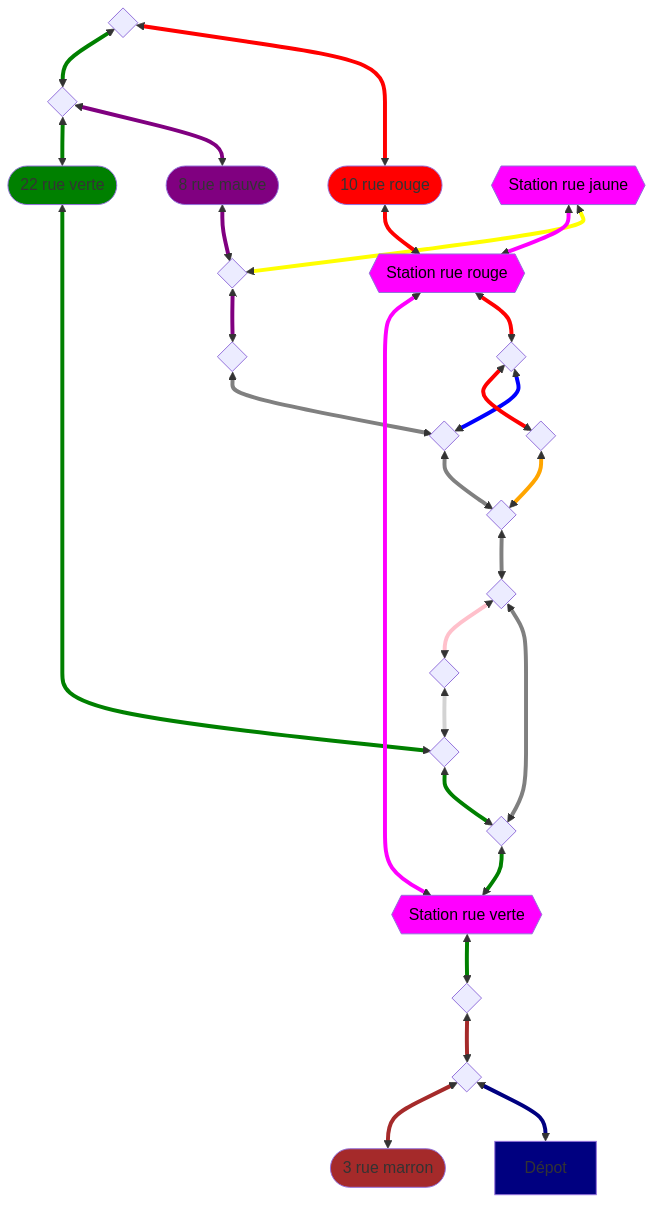
\includegraphics[height=0.7\textheight]{Images/Graph.png}
    \caption{Diagramme sagittal du graphe des adresses de livraison.
    L'utilisation de double flèches est uniquement due à des raisons techniques et équivaut à un graphe non orienté.}
    \label{fig:graphe}
\end{figure}

\clearpage

\begin{algorithm}[ht]
    \label{algo:2opt}
    \caption{Algorithme 2-opt}
    \begin{algorithmic}
    \State $T \gets \text{un tour initial}$
    \State $\text{aucun changement} \gets \text{vrai}$
    \Repeat
        \State $T_{\text{meilleur}} \gets T$
        \For{\text{toutes les paires d'arêtes possibles dans } $T$}
            \State $T' \gets \text{tour en échangeant les points finaux de la paire d'arêtes}$
            \If{$T' < T_{\text{meilleur}}$}
                \State $T_{\text{meilleur}} \gets T'$
                \State $\text{aucun changement} \gets \text{faux}$
            \EndIf
        \EndFor
        \State $T \gets T_{\text{meilleur}}$
    \Until{$\text{aucun changement est vrai}$}
    \State \Return $T$
\end{algorithmic}
\end{algorithm}

\clearpage

\begin{table}[ht]{}
    \caption{Comparaison des sorties de l'algorithme avec et sans métro}
    \label{fig:chemins}    
    \centering
    \begin{tabular}{|c|c|}
        \hline
        Avec métro & Sans métro \\
        \hline
        \begin{minipage}{6cm}
            \begin{verbatim}
Chemin optimal (19 sommets) :
=> Depot
=> Bleu_fonce_marron
=> 3_rue_marron
=> Bleu_fonce_marron
=> Marron_vert
=> Station_verte
=> Station_rouge
=> 10_rue_rouge
=> Rouge_vert
=> Mauve_vert
=> 8_rue_mauve
=> Mauve_vert
=> 22_rue_verte
=> Gris_clair_vert
=> Gris_fonce_vert
=> Station_verte
=> Marron_vert
=> Bleu_fonce_marron
=> Depot 
            \end{verbatim}
        \end{minipage}
        &
        \begin{minipage}{6cm}
            \begin{verbatim}
Chemin optimal (23 sommets) :
=> Depot
=> Bleu_fonce_marron
=> 3_rue_marron
=> Bleu_fonce_marron
=> Marron_vert
=> Station_verte
=> Gris_fonce_vert
=> Gris_clair_vert
=> 22_rue_verte
=> Mauve_vert
=> Rouge_vert
=> 10_rue_rouge
=> Rouge_vert
=> Mauve_vert
=> 8_rue_mauve
=> Mauve_vert
=> 22_rue_verte
=> Gris_clair_vert
=> Gris_fonce_vert
=> Station_verte
=> Marron_vert
=> Bleu_fonce_marron
=> Depot
            \end{verbatim}
        \end{minipage}
        \\
        \hline
    \end{tabular}
\end{table}
  
\clearpage

\printbibliography

\end{document}
